%% LaTeX2e class for student theses
%% sections/evaluation.tex
%% 
%% Karlsruhe Institute of Technology
%% Institute for Program Structures and Data Organization
%% Chair for Software Design and Quality (SDQ)
%%
%% Dr.-Ing. Erik Burger
%% burger@kit.edu
%%
%% Version 1.3.5, 2020-06-26

\chapter{Regression}
\label{ch:Regression}

After extracting features from the elements, the next step is do learn from the data.
The goal of this Bachelor's thesis is to predict the activation barrier of a catalyst molecule.
The techniques used however are not limited to the activation barrier, 
as it can be expected that other properties of the molecule could be predicted with similar techniques.

For regression, artificial neural networks(ANNs) will be used.
Neural networks have seen a huge surge in popularity in recent years for their ability to 
adapt to high dimensional input data.
The concept is derived from biological neural networks such as the ones found in the human brain.

ANNs are a composed of a set of interconnected neurons.
Each neuron has a set of inputs $x_1 .. x_n$, a bias $b$, and an activation function $f(x)$.
The output will be the result of the activation function applied to the sum of all inputs plus the bias.

$$ y = f \left( \sum_i x_i + b \right) $$

Neurons are grouped together in layers, where the output of each layer is connected to the input of the next one.
For a single prediction, the example is applied to the input layer, the network is then flooded until the output layer is reached.
In the case of regression used here, the value of the output layer is the prediction of the neural network.

% Listing 2: Tex for neural network pipeline
\begin{tikzpicture}[
    % define styles    
    init/.style={ 
         draw, 
         circle, 
         inner sep=2pt,
         font=\Huge,
         join = by -latex
    },
    squa/.style={ 
        font=\Large,
        join = by -latex
    }
]
% Top chain x1 to w1
\begin{scope}[start chain=1]
    \node[on chain=1] at (0,1.5cm)  (x1) {$x_1$};
    \node[on chain=1,join=by o-latex] (w1) {$w_1$};
\end{scope}
% Middle chain x2 to output
\begin{scope}[start chain=2]
    \node[on chain=2] (x2) {$x_2$};
    \node[on chain=2,join=by o-latex] {$w_2$};
    \node[on chain=2,init] (sigma) {$\displaystyle\Sigma$};
    \node[on chain=2,squa,label=above:{\parbox{2cm}{\centering Activation\\ function}}]   {$f_{act}$};
    \node[on chain=2,squa,label=above:Output,join=by -latex] {$y_{out}$};
\end{scope}
% Bottom chain x3 to w3
\begin{scope}[start chain=3]
    \node[on chain=3] at (0,-1.5cm) 
    (x3) {$x_3$};
    \node[on chain=3,label=below:Weights,join=by o-latex]
    (w3) {$w_3$};
\end{scope}
% Bias
\node[label=above:\parbox{2cm}{\centering Bias \\ $b$}] at (sigma|-w1) (b) {};
% Arrows joining w1, w3 and b to sigma
\draw[-latex] (w1) -- (sigma);
\draw[-latex] (w3) -- (sigma);
\draw[o-latex] (b) -- (sigma);
% left hand side brace
\draw[decorate,decoration={brace,mirror}] (x1.north west) -- node[left=10pt] {Inputs} (x3.south west);

\end{tikzpicture}



% Listing 1: Tex for neural network layers
\begin{tikzpicture}[
    % define styles 
    clear/.style={ 
        draw=none,
        fill=none
    },
    net/.style={
        matrix of nodes,
        nodes={ draw, circle, inner sep=10pt },
        nodes in empty cells,
        column sep=2cm,
        row sep=-9pt
    },
    >=latex
]
% define matrix mat to hold nodes
% using net as default style for cells
\matrix[net] (mat)
{
% Define layer headings
|[clear]| \parbox{1.3cm}{\centering Input\\layer} 
   & |[clear]| \parbox{1.3cm}{\centering Hidden\\layer} 
   & |[clear]| \parbox{1.3cm}{\centering Output\\layer} \\
        
$\alpha_{0}^{0}$  & |[clear]|        & |[clear]| \\
|[clear]|         & $\alpha_{0}^{1}$ & |[clear]| \\
$\alpha_{1}^{0}$  & |[clear]|        & |[clear]| \\
|[clear]|         & |[clear]|        & |[clear]| \phantom{$a_{0}^{0}$} \\
$\alpha_{2}^{0}$  & $\alpha_{1}^{1}$ & $\alpha_{0}^{2}$ \\
|[clear]|         & |[clear]|        & |[clear]|  \phantom{$a_{0}^{0}$} \\
$\alpha_{3}^{0}$  & |[clear]|        & |[clear]| \\
|[clear]|         & $\alpha_{2}^{1}$ & |[clear]| \\
$\alpha_{4}^{0}$  & |[clear]|        & |[clear]| \\ 
};
% left most lines into input layers
\foreach \ai in {2,4,...,10}
   \draw[<-] (mat-\ai-1) -- +(-2cm,0);
% lines from a_{i}^{0} to each a_{j}^{1}
\foreach \ai in {2,4,...,10} {
   \foreach \aii in {3,6,9}
       \draw[->] (mat-\ai-1) -- (mat-\aii-2);
       }
% lines from a_{i}^{1} to a_{0}^{2}
\foreach \ai in {3,6,9}
 \draw[->] (mat-\ai-2) -- (mat-6-3);
   
% right most line with Output label
\draw[->] (mat-6-3) -- node[above] {Output} +(2cm,0);
\end{tikzpicture}

Finding the right amount of layers and the right type of activation functions is a challenging part of neural network.
Since generally no rule is known on what neural network architecture will work best on the given data, the space of possible networks needs to be explored.
A variety of choices for the network architecture can be made, such as the amount of layers, size of the layers, type of activation functions, regularization, normalization, and many more.

When choosing the network architecture, generally a bigger network will be able to adapt to the data better.
However if the network will become to big, it might encounter issues with overfitting.
Overfitting is a problem encountered when the network adapts to the training data too well.
This will decrease it's ability to generalize the data and make good predictions on previously unseen samples \ref{fig:overfitting}.

A measure to counteract overfitting is regularization.
Regularization introduces a penalty term that punishes the network for extreme values.
Specifically a regularization parameter $\lambda$ is introduced.
When training the network a regularization term for every weight $w_i$ is added to the loss function.

$$
Loss_{regularized} = Loss +  \sum_i \lambda_i \cdot w_i^2 
$$

When the training algorithm calculates the derivative of the regularized loss function, it will generally gravitate towards smaller weights.
Flatter weights result in a flatter regression reducing the ability of the noise to adapt to small noise in the input data.
The hope is that outliers in the training data will be ignored and the relevant data will be abstracted.
In theory, a regularization parameter $\lambda$ could be defined for every weight in the network.
In practice, all weights in one layer are assigned the same regularization parameter.


\begin{figure} [h]
    \centering
    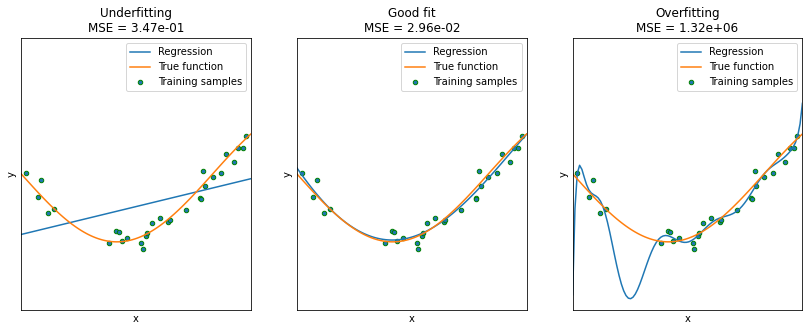
\includegraphics[width=0.9\textwidth]{figures/regression/overfitting.png} 
    \caption{Regression on a function with training examples. 
            The underfitting model is not complex enough to fit to the data well. 
            The overfitting model is too complex for the data.
            While the training error is lower for the overfitting model, 
            the overall performance of the overfitting model on previously unseen data 
            is worse than for the model with a good fit.
        }
    \label{fig:overfitting}
\end{figure}
  
To prevent overfitting while still getting good regression results, multiple network architectures need to be considered.
The networks proposed here were found by trail and error first, and later improved by hyperparameter analysis.

%TODO: Introduce NNs, normalzation, regularization, overfitting, underfitting.
% TODO: Regularization
% TODO: Normaliztation blabla

\section{Regression on fourier descriptor features}
\label{sec:Evaluation:fourier}

In the first approach, the features generated by the fourier descriptor were used to training.
Notable hyperparameters to the feature extractor here are the number of layers $l$ and the order of the fourier descriptor $o$.

The start and end height of the layers are chosen so that all the molecules in the dataset fully fit within $z_{min}$ and $z_{max}$.

The output shape of the descriptor will be an array of size $l \times (o * 4 - 1)$.
Generally, the bigger the number of fourier coefficients, the better the contour can be approximated.
However, an order that is chosen too high may increase the risk of overfitting, 
This problem is commonly referred to as "the curse of dimensionality".

A simple numerical approach to finding the order with the highest prediction accuracy is not necessarily viable in this case.
Since the ultimate goal is not to get the most accurate prediction possible, but instead discover which parts of 3d space 
are responsible for prediction, an order that offerers reasonable high accuracy without being subject too to much noise when explaining the 
prediction needs to be found. %TODO: Other reasons why order 10?

After various tests with multiple orders, an order of $k_{max} = 10$ seemed to be a good compromise between accuracy of description and accuracy of prediction.

The same problem is faced when defining the number of slices.
Here the problem becomes more tricky, since the number of slices seems to play a huge part in the architecture of the ANN used.
While the minimal number of slices should also be defined manually to allow for a proper reconstruction, the exact number of slices should be subject of a hyperparamter analysis.

%TODO: Hyperparameter analysis

Since every slice is composed of same kind of fourier coefficients, the first idea was to use convolution layers the decrease the dimensionality of the input.
Filters might be able to recognize structures in each of the slices, and applied them across the different slices.

Convolution layers heavily depend on the assumption that the relative location of features in matters.
Filter sizes were therefor chosen to correspond to the dimensions over which similarities in the structures of the features are expected.
In the case of fourier coefficients, the filter therefor were only stretched along the layer dimension, and not along the dimension of the fourier descriptors.

Multiple tests were performed with various filter sizes and convolution layers.
The regression accuracy was falling short of expectations, and the general shape of the network did not seem to change the prediction accuracy significantly.

\begin{figure} [h]
    \centering
    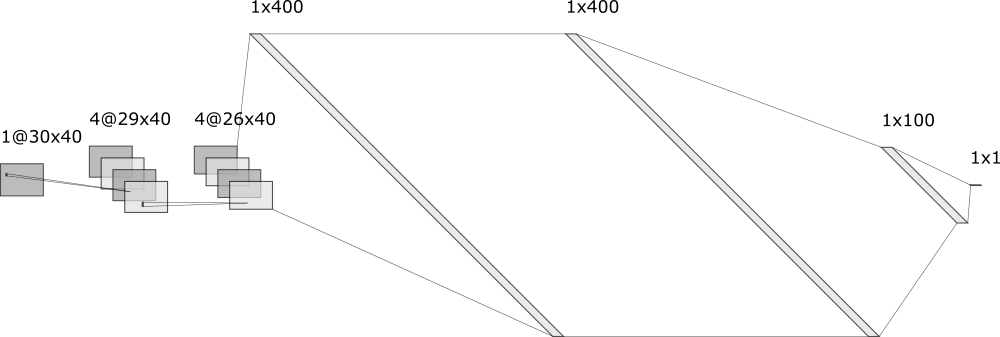
\includegraphics[width=0.7\textwidth]{figures/regression/fourier/cnn/fourier_conv_layout.png} 
    \caption{
        Architecture of the convolutional neural network used for predicting the activation barrier from fourier coefficients.
    }
    \label{fig:cnn-architecture}
\end{figure}

In first network architectures, overfitting was a mayor problem.
With regularization and other techniques the issue of overfitting could be reduced.
What became clear pretty early in the tests was that convolution layers did not improve prediction accuracy as expected.
When testing different filter configurations, the network performed best the smaller the filters got, and the fewer convolution layers were used.
In the end, the best performing Convolutional Neural Network found had two Convolution Steps with a filter size of $2 \times 1$ for the first layer, and a filter size
of $4 \times 1$ for the second layer \ref{fig:cnn-architecture}.
After the convolution layers 3 fully connected layers and the output layer followed.
Dropout and batch normalization layers were added in between to help with fighting overfitting.
The prediction accuracy of the CNN was similar yet slightly worse than the prediction accuracy achieved on autocorrelation features \cite{friederich_dos}.
The best CNN achieved a mean squared error over all test examples of $MAE=1.36$ and a coefficient of determination of $r^2=0.84$ \ref{fig:fourier_cnn}.
In comparison, the best neural network of \cite{friederich_dos} achieved a prediction accuracy of $MAE=1.12$ and $r^2=0.845$.

Since the space of possible network configurations is highly irregular, there is likely a network configuration using convolution layers 
that performs better than the one found here.
However all the tests performed were indicating that densely connected layers would achieve similar or higher accuracy.
The idea of convolution layers was therefore dropped early on, and instead the focus was shifted to optimizing a fully-connected architecture.

\begin{figure}[!htb]
    \minipage{0.1\textwidth}
    \endminipage\hfill
    \minipage{0.4\textwidth}
      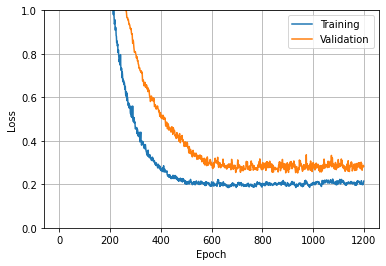
\includegraphics[width=1.0\textwidth]{figures/regression/fourier/cnn/lossCNN.png}
    \endminipage\hfill
    \minipage{0.4\textwidth}
      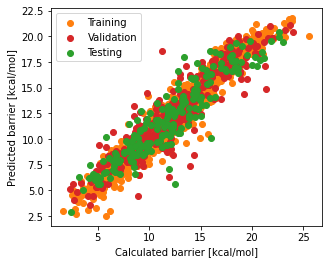
\includegraphics[width=1.0\textwidth]{figures/regression/fourier/cnn/scatterCNN.png}
    \endminipage\hfill
    \minipage{0.1\textwidth}
    \endminipage
    \caption{
        Loss while training the CNN. The jitter in the training loss during convergence is likely caused by the dropout layers. 
        The optimization goal was minimizing the mean squared error. 
        Training was performed on 80\% of the data.
        On the right are the predictions of the activation barrier in comparison to the real values ($MAE=1.36$, $r^2=0.84$).
    }
    \label{fig:fourier_cnn}
\end{figure}

Since previous research has proven that similar accuracy to the convolution approach can be achieved by learning from autocorrelation features,
the next idea was to use a transfer learning approach.
In a first step, the network would be taught to predict the autocorrelation features computed in \cite{friederich_dos}.
In a second step, the network is then extended to learn to predict that activation barrier \ref{fig:transferlearn}.
The hope was that teaching the network about autocorrelation features, the model would learn to recognize relevant properties of a catalyst.
In a second step, the entire network would then be trained to adapt specifically to the activation barrier.

\begin{figure} [h]
    \centering
    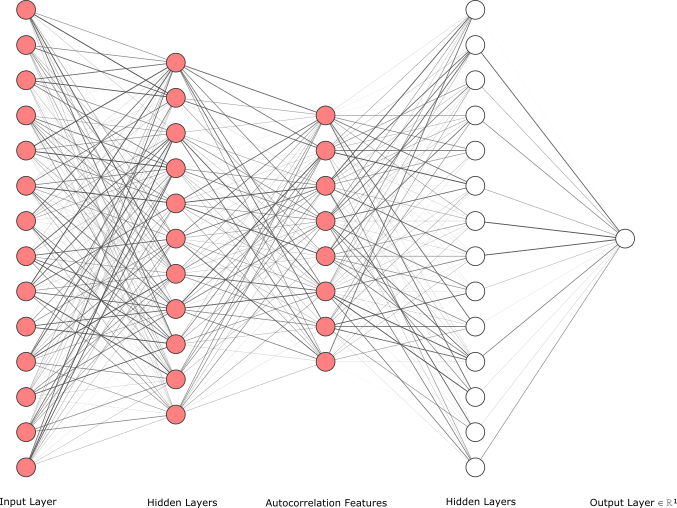
\includegraphics[width=0.7\textwidth]{figures/regression/fourier/nn.png} 
    \caption{Illustration of the transfer learning approach.
        In red the original model predicting autocorrelation features from the input is illustrated.
        In white the second part of the network, predicting the activation barrier from the autocorrelation features, is illustrated.
        Different sizes and amounts of hidden layers were tested. Here, single hidden layers are shown for illustration purposes.
    }
    \label{fig:transferlearn}
\end{figure}

Since the convolutional approach did not seem to improve results, a fully connected architecture predicting autocorrelation features from fourier coefficients 
was used.
Since there were 30 autocorrelation features used, the last layer of the network had a size of 30.
Findings about good hyperparameter, such as layer size, regularization and dropout rates, could be partly reused from the convolution step.
In the end, a network that predicted 30 independent autocorrelation features was found.
The network was able to predict some autocorrelation with very high accuracy. Specifically, the $T$ features and $I$ features were
predicted with an accuracy of $r^2 > 0.98$. 
Other features, such as $Z$ features, were lacking behind in accuracy, with the network only being able to reach accuracy of $r^2<0.96$ for some features.
The features the network was able to approximate well were also less important to the network found in \cite{friederich_dos}, while the features 
the network performed poorly on were the more important features \ref{fig:transfer_result}.

\begin{figure}[!htb]
    \minipage{0.32\textwidth}
      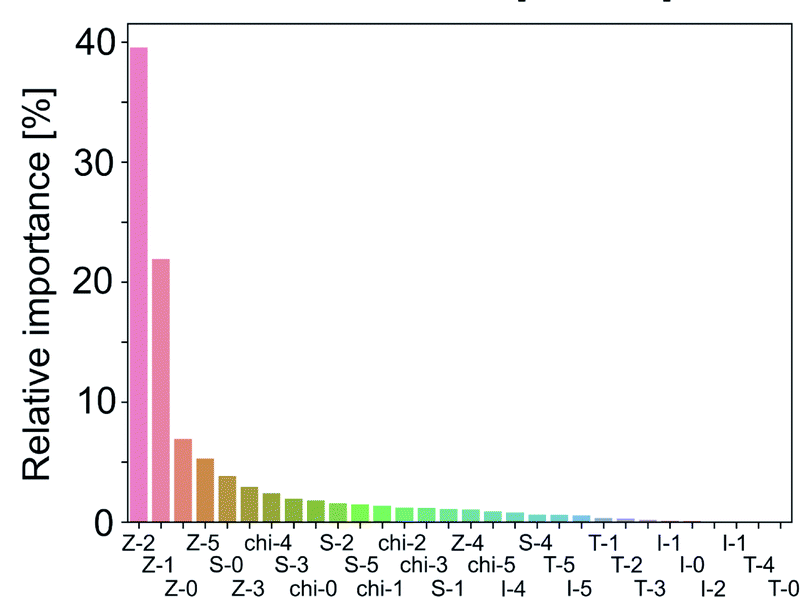
\includegraphics[width=1.0\textwidth]{figures/regression/fourier/importance_map.png}
    \endminipage\hfill
    \minipage{0.32\textwidth}
      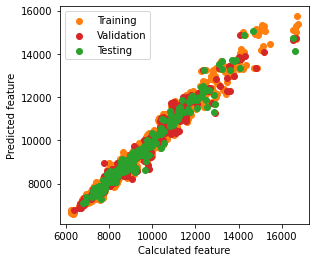
\includegraphics[width=1.0\textwidth]{figures/regression/fourier/transfer/scatterZ2.png}
    \endminipage
    \minipage{0.32\textwidth}
      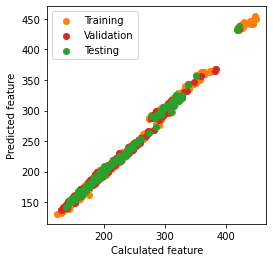
\includegraphics[width=1.0\textwidth]{figures/regression/fourier/transfer/scatterT0.png}
    \endminipage
    \caption{
    Left: Importance of features for the neural networks discussed in \cite{friederich_dos}.
    Middle: Prediction of Z-2 features from fourier features.
    Right: Prediction of T-0 features from fourier features. 
    The network was trained on 80\% of the data points.
    }
    \label{fig:transfer_result}
\end{figure}

After the network predicting the autocorrelation features was trained, the the transfer learning was started.
The last layers of model were removed, and replaced with newly initialized layers.
These newly added layers have and output size of 1 to allow for prediction of the activation barrier.
The best configuration found kept the first 3 layers of the original network, and then added 3 additional hidden layers and one output layer.
Regularization and normalization was used for some of the layers.
The model was then trained again with fourier coefficients as input and activation barriers as output.
Compared the convolution approach, the network took longer to converge, the overall regression accuracy improved.
The network achieved a $r^2=0.874$ and a $MAE=1.139$ when trained on 80\% of the data \ref{fig:transfer_final}.

\begin{figure}[!htb]
    \minipage{0.3333\textwidth}
      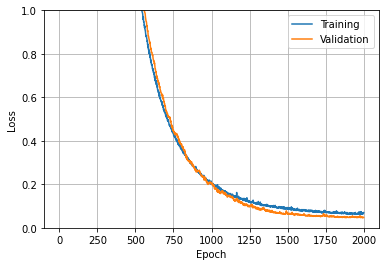
\includegraphics[width=1.0\textwidth]{figures/regression/fourier/transfer/lossTransferAutocor.png}
    \endminipage\hfill
    \minipage{0.3333\textwidth}
      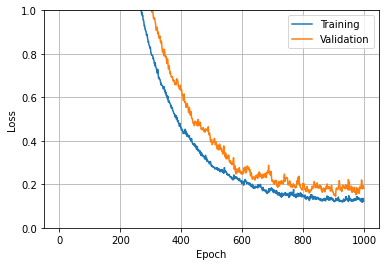
\includegraphics[width=1.0\textwidth]{figures/regression/fourier/transfer/lossTransferFull.png}
    \endminipage\hfill
    \minipage{0.3333\textwidth}
      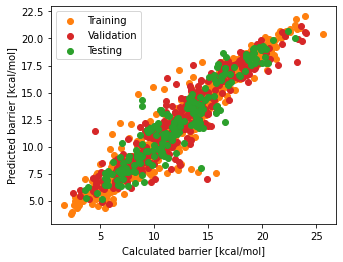
\includegraphics[width=1.0\textwidth]{figures/regression/fourier/transfer/scatterTransferFull.png}
    \endminipage
    \caption{
    Loss of the network being trained to predict autocorrelation features (right).
    The adapted network is then trained again to predict the activation barrier. The loss function in the middle shows the second training.
    The prediction accuracy has slight improved (right).  
    }
    \label{fig:transfer_final}
\end{figure}

In an attempt to find a better network architecture, a hyperparameter optimization was performed.
Hyperparameter optimization is a way of finding good hyperparameter for the underlying problem.
A searchspace need to be defined manually first, an optimization algorithm is then run to find good parameters within the search space.
Generally a bigger search space mean longer computation time for the hyperparameter algorithm.
The search space here was limited by the findings of manual hyperparamter tuning.
Notable optimization values given to the hyperparamter tuner were the number of convolution layers, 
the number and size of fully connected layers, the regularization rate of these layers, and the dropout rate for the layers.


\begin{figure}[!htb]
    \minipage{0.3333\textwidth}
      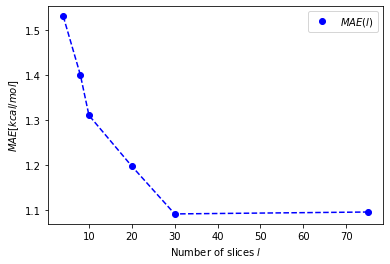
\includegraphics[width=1.0\textwidth]{figures/regression/fourier/mae_layer.png}
    \endminipage\hfill
    \minipage{0.3333\textwidth}
      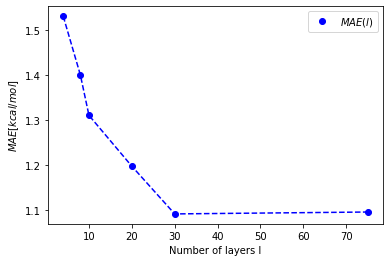
\includegraphics[width=1.0\textwidth]{figures/regression/fourier/r2_layer.png}
    \endminipage\hfill
    \minipage{0.3333\textwidth}
      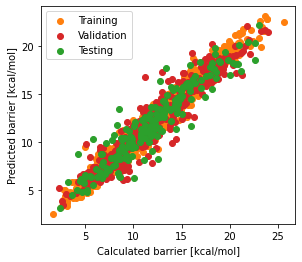
\includegraphics[width=1.0\textwidth]{figures/regression/fourier/scatterHyperparam.png}
    \endminipage
    \caption{
    The $r^2$ values and $MAE$ for different layer heights.
    For all layer heights a separate hyperparameter optimization wa run, resulting in different network architectures.
    All networks are trained using 80\% on the data. The $r^2$ scores and $MAE$ were evaluated later using a test dataset.
    The on the right the prediction of the best performing network found in the hyperparameter optimization step is plotted.
    The best network was found using a input layer height of $0.2 \AA$ resulting in $75$ layers. 
    The $MAE=1.096$ and $r^2=0.882$ are the highest accuracy so far.
    }
    \label{fig:fourier_final}
\end{figure}


In addition, multiple hyperparameter optimizations were performed for different layer heights $l$.
Since the layer heigh also changes the input size of the neural network, an assumption about the 
architecture across different layer heights is not feasible.
For ever layer height a separate hyperparamter optimization was run \ref{fig:fourier_final}.
The best hyperparameters found for every input site vary substantially.

After a certain layer height the prediction accuracy seems to no longer improve.
The step from 30 to 75 layers does not change the accuracy significancy, while more than doubling input size.
The small improvement in accuracy from 30 to 75 layers might not necessarily mean a higher overall classification accuracy of the network,
but could also be to randomness when selecting training and test examples or randomness during training.

The process shows that performing regression on fourier features is possible.
The accuracy however is not significantly higher than the accuracy achieved on graph convolutions.
Since the goal of this thesis is to learn from the 3D structure of the molecule, the similar performance 
indicates that the information learned from the 3d structure is limited.
This assumption is further validated by the fact that the transfer learning approach that 
basically eliminates spacial information about the network in the middle of the network, achieves similar accuracy to the 
network trained on features that do not include any information about the 3d structure.

Due to these results, a different feature extractor, SNAP, was developed.

\section{Regression on SNAP features}
\label{sec:Evaluation:snap}

Similar to the feature space for fourier coefficients, the size of the SNAP feature space is determined by two factors.
The first is the number of elements in the dataset.
The second is the resolution of the encoding for each type of element, defined by $n_{max}$ and $l_{max}$.

Other hyperparameters, such as the choice of radial basis functions, might influence the prediction accuracy further.

The number of radial basis functions $n_{max}$ and the maximum degree of spherical harmonics $l_{max}$ do both influence
the input dimension.
The ideal network architecture for different values will therefor vary too.
Since the values determine the accuracy with which accuracy the space is encoded, choosing these values purely 
based on which combination achieves the highest classification accuracy is not feasible.
The higher the degree of the spherical harmonics and radial basis functions, the more precise the element can be described.
The higher number of coefficients might however come at the price of noise when trying to explain the prediction later on.
A good balance between interpretability and accuracy was found with $l_{max}=n_{max}=3$. %TODO: Really? 

Hyperparameter analysis was performed on different combinations of $n_{max}$, $l_{max}$.
Since hyperparameter optimization is very computationally expensive, taking up to multiple days on modern high-performance 
server hardware, the number of combinations that could be explored is limited.

\subsection{Normalization}

In a first step, the features generated by SNAP and the labels were normalized.
Normalize means scaling both labels and features independently so that mean is equal to $0$ and the standard deviation is equal to $1$.
Normalization is performed on each feature independently of each other.
This helps the network to generalize from the data better since no large biases have to be learned.

Since the data is normalized, the output from the network will not be the activation barrier directly.
Instead, the output needs to be scaled back to compute the performance of the network.

\subsection{Convolutional Neural Network}

Similar to the features generated by EFD, the output of SNAP can be shaped into a feature matrix again.
Here, each layer will correspond to one species of atoms.
Since the dataset the model is trained on consists of 12 different species of atoms, the feature matrix will have a height of 12.
Each row will then hold the coefficients describing the density of this species around the iridium center.
Depending on the choice of $n_{max}$ and $l_{max}$, the number of coefficients will change.

Since a coefficient of the $k$-th row will correspond to $c^k_{nlm}$, meaning every coefficient in the same colum has the same spacial meaning,
a convolutional neural network was the first idea to reduce the size of the input space and allow the network to learn structure in the input data.

Since not every molecule in the dataset consists of every atom, the input matrix will generally be sparse.
Rows that correspond to atoms not in the dataset will be filled with 0.
A filter that learns the general structure of the space and that is moved over the different species, therefor 
being able to ignore sparse inputs seemed to be a good choice.

Using a hyperparameter optimization to find the ideal filter size and number of convolution layers however showed
the a fully connected approach reaches higher accuracy than convolutional layers.
The hyperparameter optimizer not only gravitated towards a small amount of filters, but also towards 
the smallest possible filter size allowed in the hyperparameter space.

In further optimization the idea of convolution layers was therefor dropped in favour of fully connected layers.

\subsection{Fully connected neural network}


\section{Comparison}
\label{sec:Evaluation:Comparison}

\dots
%% ---------------------
%% | / Example content |
%% ---------------------